\subsection{Abstraction and Automation}
  \noindent
  \marginnote{3.4.1.1}Problem solving is the process of finding solutions to a certain problem. One of the main tools used when problem solving is the application of Logical Reasoning which is the process of using a given set of facts to determine whether new facts are true or false. To solve a problem another important step is to identify what the problem is.\\ \\
  \marginnote{3.4.1.2}An Algorithm is a sequence of steps that can be followed to complete a task and that always terminate. An example of an algorithm (written in pseudo-code) is as follows:
  \begin{python}
func bubblesort( var a as array )
for i from 1 to N
	for j from 0 to N - 1
	  if a[j] > a[j + 1]
	    swap( a[j], a[j + 1] )
end func
  \end{python}
  We can use a technique called hand-tracing/ dry running to work through the code and see if it works as intended. An example of a dry run is as follows:
  \begin{table}[H]
    \centering
    \begin{tabular}{| C{2cm} | C{2cm} | C{2cm} C{2cm} C{2cm} C{2cm} |}
      \hline
      \textbf{i} & \textbf{j} & \multicolumn{4}{c|}{\textbf{a}} \\
      \hline
      0 & 0 & 3 & 2 & 1 & 4 \\
      \cline{3-6}
      1 & 0 & 2 & 3 & 1 & 4 \\
      \cline{3-6}
      1 & 1 & 2 & 1 & 3 & 4 \\
      \cline{3-6}
      1 & 2 & 2 & 1 & 3 & 4 \\
      \cline{3-6}
      2 & 0 & 1 & 2 & 3 & 4 \\
      \cline{3-6}
      2 & 1 & 1 & 2 & 3 & 4 \\
      \cline{3-6}
      2 & 2 & 1 & 2 & 3 & 4 \\
      \cline{3-6}
      3 & 0 & 1 & 2 & 3 & 4 \\
      \cline{3-6}
      3 & 1 & 1 & 2 & 3 & 4 \\
      \cline{3-6}
      3 & 2 & 1 & 2 & 3 & 4 \\
      \hline
    \end{tabular}
  \end{table}
  \noindent
  This shows what happens to the data throughout the process at which the algorithm is being run.\\ \\
  \marginnote{3.4.1.3}The main concept behind abstraction is to reduce a problem to its most basic parts, its essential features. This is useful as it allows a programmer to solve the problem without having to fuss too much about the details, abstraction is also useful because it allows the solution to one problem to be implemented in other similar problems. In general, there are two main types of abstraction:
  \begin{itemize}
    \setlength{\itemsep}{0em}
    \item Representational Abstraction
    \begin{itemize}
      \setlength{\itemsep}{0em}
      \item This is the process of removing unnecessary details so that only information that is required to solve the problem remains. An example of this is a train map, as this shows how the different stations are connected, but doesn't really care about actual distance or time taken.
    \end{itemize}
    \item Abstraction by generalisation/categorisation
    \begin{itemize}
      \setlength{\itemsep}{0em}
      \item This is the concept of reducing problems by putting aspects of a problem into hierarchical categories using an "is a kind of" relationship. An example of this is could be a tree showing the different sciences, e.g:
    \end{itemize}
  \end{itemize}
  \begin{center}
    \begin{tikzpicture}[
    level 1/.append style={level distance=2cm},
    level 2/.append style={level distance=2cm}]
    \tikzstyle{every node}=[rectangle, rounded corners, minimum width=2cm, minimum height=1cm,text centered, draw=black]
    \Tree
    [.Science
      [.{Mathematics}
          [.{Applied Mathematics}	]
          [.{Pure Mathematics} ]
      ]
      [.{Physics} ]
      [.{Chemistry} ]
      [.{Biology} ]
    ]
    \end{tikzpicture}
  \end{center}
  \marginnote{3.4.1.4}The process of information hiding involves hiding all details about an object that do not contribute to its essential characteristics. A simple example of this is using a car, as you can control it by using the steering wheel, gearbox, pedals, etc. and don't need to know the mechanics behind it.\\
  There are many different types of abstractions, for example:
  \begin{itemize}
    \setlength{\itemsep}{0em}
    \item \marginnote{3.4.1.5}Procedural Abstraction
    \subitem This is the concept that all solutions can be broken down into a series of procedures, an example would be a recipe.
    \item \marginnote{3.4.1.6}Functional Abstraction
    \subitem This is the concept that all solutions can be broken down into reusable functions. Functions can be thought of as abstracted procedures as one can call a function without completely knows how it works.
    \item \marginnote{3.4.1.7}Data Abstraction
    \subitem This is the concept of hiding how a data type is represented, making it easier to construct new data objects (called compound data objects). It also involves separating implementations of data objects and the user interface.
    \item \marginnote{3.4.1.8}Problem Abstraction/ Reduction
    \subitem This is the process of removing unnecessary details in a problem until the underlying problem is identified to see if this is the same as a problem that has already been solved.
  \end{itemize}
  \marginnote{3.4.1.9}Decomposition is the process of breaking a large task into a series of subtasks. Procedural decomposition is the process of breaking down a task into procedures and subroutines.\\
  \marginnote{3.4.1.10}Composition is the building up of a whole system from smaller units. The opposite of decomposition. This involves:
  \begin{itemize}
    \setlength{\itemsep}{0em}
    \item Writing all the procedures and linking them together to create compound procedures.
    \item Creating data structures and combining them to form compound structures.
  \end{itemize}
  \begin{center}
    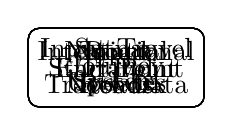
\begin{tikzpicture}[
    level 1/.append style={level distance=2cm},
    level 2/.append style={level distance=2cm}]
    \tikzstyle{every node}=[rectangle, rounded corners, text width=2cm,  minimum width=2cm, minimum height=1cm,text centered, draw=black]
    \Tree
    [.\node[anchor=north west](a){Satnav System};
      [.\node[anchor=north west](b){Journey};
        [.\node[anchor=north west](c){Start Point};	]
        [.\node[anchor=north west](d){End Point}; ]
      ]
      [.\node[anchor=north west](e){Travel};
        [.\node[anchor=north west](f){Input Travel Data};	]
        [.\node[anchor=north west](g){Input Travel Updates}; ]
      ]
      [.\node[anchor=north west](h){Road Network};
        [.\node[anchor=north west](i){National Roads};	]
        [.\node[anchor=north west](j){International Roads}; ]
      ]
    ]
    %\node(k)[below=6cm]{Calculate Route};
    %\draw (c.south) -| (k);
    %\draw (d.south) -| (k);
    %\draw (f.south) -| (k);
    %\draw (g.south) -| (k);
    %\draw (i.south) -| (k);
    %\draw (j.south) -| (k);
    \end{tikzpicture}
  \end{center}
  \marginnote{3.4.1.11}Automation is the process of creating computer models (abstraction of real world objects/ phenomena) of real-life situations and putting them into action to solve problems. This is done by:
  \begin{itemize}
    \setlength{\itemsep}{0em}
    \item Understanding the problem.
    \item Creating Algorithm.
    \item Implementing the algorithms in program code.
    \item Implementing the models in data structures.
    \item Executing the code.
  \end{itemize}
\subsection{Regular Languages}
  \noindent
  \marginnote{3.4.2.1}A finite state machine is any device device that stores its current state and whose status can change as the result of an input. Mainly used as a conceptual model for designing and describing systems. A state transition diagram is a visual representation of an FSM using circles and arrows, whereas a state transition table is a tabular representation of an FSM showing input, current state, and next state. Within a state transition diagram, there may be an accepting state, represented by two concentric circles, which shows whether an input has been accepted. An FSM doesn't necessarily need an accepting state. Below is an example of both a state transition diagram and a state transition table.\\
  \begin{figure}[H]
    \centering
    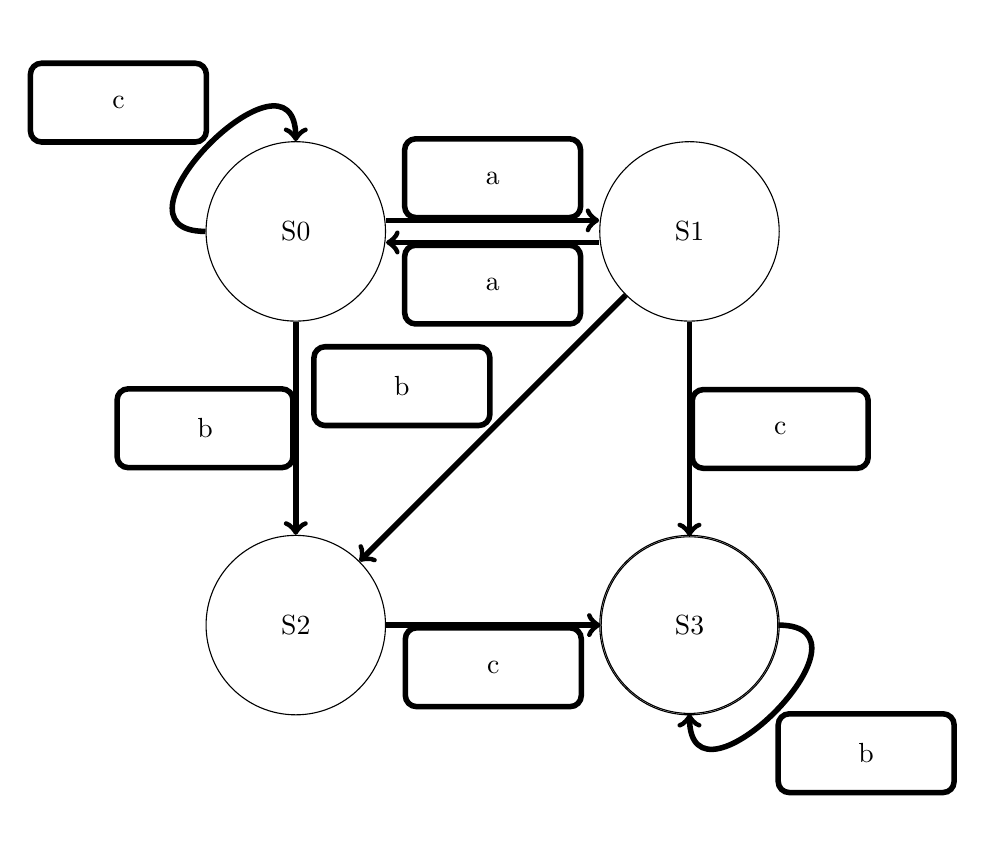
\begin{tikzpicture}
      \def \n {5};
      \node[circle, minimum width=1cm, draw=black](S0) at (0,\n) {S0};
      \node[circle, minimum width=1cm, draw=black](S1) at (\n,\n) {S1};
      \node[circle, minimum width=1cm, draw=black](S2) at (0,0) {S2};
      \node[circle, minimum width=1cm, draw=black](S3) at (\n,0) {S3};
      \node[circle, minimum width=1.2cm, draw=black](S4) at (\n,0) {};

      \draw[->, line width=2pt] ([yshift= 4pt]S0.east) -- node[above] {a} ([yshift= 4pt]S1.west);
      \draw[->, line width=2pt] (S0.south) -- node[left] {b} (S2.north);
      \draw[->, line width=2pt] ([yshift= -4pt]S1.west) -- node[below] {a} ([yshift= -4pt]S0.east);
      \draw[->, line width=2pt] (S1.south west) -- node[above left] {b} (S2.north east) ;
      \draw[->, line width=2pt] (S1.south) -- node[right] {c} (S4.north);
      \draw[->, line width=2pt] (S2.east) -- node[below] {c} (S4.west);
      \draw[->, line width=2pt] (S4.east) .. controls ([xshift= 40pt]S4.east) and ([yshift= -40pt]S4.south) .. node[below right] {b} (S4.south);
      \draw[->, line width=2pt] (S0.west) .. controls ([xshift= -40pt]S0.west) and ([yshift= 40pt]S0.north) .. node[above left] {c} (S0.north);
    \end{tikzpicture}
    \caption*{State Transition Diagram}
  \end{figure}
  \begin{figure}[H]
    \centering
    \begin{tabular}{| C{4cm} | C{4cm} | C{4cm} |}
      \hline
      Input & Current State & Next State \\
      \hline
      c & S0 & S0 \\
      a & S0 & S1 \\
      b & S0 & S2 \\
      a & S1 & S0 \\
      b & S1 & S2 \\
      c & S1 & S3 \\
      c & S2 & S3 \\
      b & S3 & S3 \\
      \hline
    \end{tabular}
    \caption*{State Transition Table}
  \end{figure}
  A Mealy Machine is a type of finite state machine which also produces an output, this output can be shown on a diagram by instead of labelling each transition with ``input'', you label them with ``input/output'', and that output is outputted when the transition it is on occurs. This can also be represented in a state transition Table by simply adding a column.\\ \\
  \noindent
  \marginnote{4.4.2.2}There is a lot of random maths that is part of this course that isn't taught as part of even standard A level maths, but thankfully it only covers basic concepts so. The first thing we need to do is define a set, a set is ``a well-defined collection of distinct objects'', as we are only likely to deal with real numbers, you can just think of it as a collection of different numbers (they don't need to be in any specific order). A set is often defined using curly brackets for example, a set called A which is the set of numbers 1,2,3,4,5 would be shown as $A = {1,2,3,4,5}$.
  There are a few standard sets that you should know
  \begin{itemize}
  	\item Real - The set of all numbers on the number line, represented as $\mathbb{R}$
  	\item Rational - the set of all numbers that can be expressed as $\frac{a}{b}$ where $a$ and $b$ are both integers, represented as $\mathbb{Q}$
  	\item Integers - The set of all whole numbers, positive and negative, represented as $\mathbb{Z}$
	  	\subitem $\mathbb{Z} = \{\dots,-3,-2,-1,0,1,2,3,\dots\}$
  	\item Naturals - The set of all positive, whole numbers, represented as $\mathbb{N}$
	  	\subitem $\mathbb{N} = \{0,1,2,3,4,5,6,\dots\}$
  \end{itemize}
  
  There are other ways to define a set instead of just listing the numbers, you can instead define how the set should be built, this is called set comprehension/ set building. for example set $B=\{x^2 \mid x\in\mathbb{N} \wedge x \geq 2\}$
  Could be broken down as follows:
  \begin{itemize}
  	\item B - the name of the set
  	\item \{\} - indicates the contents of the set
  	\item $x^2$ - This indicates the values which you put into the set
  	\item $\mid$ - Such that, the part after this defines the values which x can take
  	\item $\in$ - is a member of
	\item $\mathbb{N}$ - The set of natural numbers
	\item $\wedge$ - and 
	\item $\geq2$ - greater than or equal to 2
  \end{itemize}
  So to write it as one sentence, the set B is the set of all values of $x^2$ such that x is a member of the set of natural numbers, and x is greater than or equal to 2. ($B=\{4,9,16,25,36,49,64,\dots\}$). One of the more unique and important sets is the empty set ($\{\} = \varnothing$) which contains no elements. Often is is easier to use a set comprehension to define a set, especially if it is infinite, for example the set $\{0^n1^n \mid n \geq 1\} = {01,0011,000111,00001111,0000011111,\dots}$. In python, sets are also defined using curly brackets.
  
When talking about a set, it can be either finite or infinite. A finite set is a set that has a finite number of elements, it has an upper limit (less than infinity), whereas an infinite set has an infinite number of elements, it is not finite. A set is said to be countable if it has the same cardinality as some subset of the natural numbers, or more simply put, if it can be counted using the natural numbers. This implies that all finite sets are countable, as well as sets with the same cardinality (size) as the natural numbers. This brings us onto countably infinite sets, these are infinite sets that are countable, this means the set has the same cardinality as natural numbers, implying that the set and natural numbers can me mapped in a way to form a one to one correspondence between each elements of the two sets (for an example, look up Cantor's diagonal argument). The cardinality of a set is the number of elements within the set.
  
  There are 5 set operations that you need to know:
  \begin{itemize}
  	\item Cartesian Product - Combines 2 sets to create a set of ordered pairs, for example, if $A=\{a,b,c\}$ and $B=\{1,2,3\}$ then $A\times B = \{
  	\left(a,1\right)
  	\left(a,2\right)
  	\left(a,3\right)
  	\left(b,1\right)
  	\left(b,2\right)
  	\left(b,3\right)
  	\left(c,1\right)
  	\left(c,2\right)
  	\left(c,3\right)
  	\}$ to define more generally, $A \times B = \{(x,y) \mid x \in A \wedge y \in B\}$.
  	\item Membership - This is when an element belongs to a set so for example if we had a set $A=\{1,2,3,4\}$ then we can say that 2 is a member of the set A or in set notation $2\in A$
  	
  	\item Union - This joins two sets together so that it contains all of the elements that are in each of the sets. For example, the union of the set $A=\{1,2,3,4\}$ and the set $B=\{3,4,5,6\}$ is $\{1,2,3,4,5,6\}$ or in set notation $A \cup B = \{1,2,3,4,5,6\}$. It can be thought of as an OR.
  	
  	\item Intersection - This joins two sets together so that it contains all of the elements that are in both sets. For example, the intersection of the set $A=\{1,2,3,4\}$ and the set $B=\{3,4,5,6\}$ is $\{3,4\}$ or in set notation $A \cap B = \{3,4\}$ . It can be though of as an AND.
  	
  	\item Difference - This joins two sets together so that it contains all of the elements that are in one of the sets, but not in both sets. For example, the difference of the set $A=\{1,2,3,4\}$ and the set $B=\{3,4,5,6\}$ is $\{1,2\}$ or in set notation $A - B = \{1,2\}$ also $B - A = \{5,6\}$. The symmetric difference is $(A - B)\cup(B - A) = A \ominus B = A \Delta B = {1,2,5,6}$ (in our example).
  \end{itemize}
  
  A set $A$ is a subset of another set $B$ if all elements of the set $A$ are elements of the set $B$. In other words, the set $A$ is contained inside the set $B$. The subset relationship is denoted as $A\subseteq B$. For example if $A = \{2,3,4\}$ and $B = \{1,2,3,4,5\}$ then $A\subseteq B$, this would also be true if $A = \{1,2,3,4,5\}$. A set is $A$ proper subset of $B$ if A is a subset of $B$ and $A \neq B$, so for example,  if $A = \{2,3,4\}$ and $B = \{1,2,3,4,5\}$ then $A\subset B$, this would not also be true if $A = \{1,2,3,4,5\}$ as $A=B$ therefore $A$ can't be a proper subset of $B$.\\ \\
  \noindent
  \marginnote{4.4.2.3}A regular expression is a simple way of describing a set and allow convenient shorthand description of certain languages. Here are common regular expressions:
  \begin{table}[H]
  	\begin{tabular}{l | l | l}
  		Regular Expression & Meaning & Strings Produced \\\hline
  		abc         & a then b then c                 & abc \\\hline
  		a|b|c       & a or b or c                     & a \\
	  	            &                                 & b \\
	  	            &                                 & c \\\hline
	  	a*bc        & 0 or more a then b then c       & bc\\
	  	            &                                 & abc \\
	  	            &                                 & aabc \\
	  	            &                                 & aaabc \\\hline
	  	a+bc        & 1 or more a then b then c       & abc \\
	  	            &                                 & aabc \\
	  	            &                                 & aaabc \\\hline
	    a?bc        & 0 or 1 a then b then c          & bc \\
	                &                                 & abc \\\hline
	    a\{2,5\}bc  & 2 to 5 a then b then c          & aabc \\
	                &                                 & aaabc \\
	                &                                 & aaaabc \\
	                &                                 & aaaaabc \\\hline
	  	(a|b)c      & a or b, then c                  & ac \\
	  	            &                                 & bc \\\hline
	  	.bc         & any character then b then c     & abc\\
	  	            &                                 & bbc\\
	  	            &                                 & cbc\\
	  	            &                                 & dbc\\
	  	            &                                 & 1bc\\\hline
	  	[abc]bc     & a or b or c then b then c       & abc \\
	  	            &                                 & bbc \\
	  	            &                                 & cbc \\\hline
	  	[\^ abc]bc   & (not a or b or c) then b then c & dbc \\
	  	            &                                 & ebc \\
	  	            &                                 & 1bc \\\hline    
  	\end{tabular}
  \end{table}
  
  Regular expressions can also be represented using a finite state machine, for example, the regular expression a*(b|c)(bc)* could be represented by the following finite state machine.
  
  \begin{figure}[H]
  	\centering
  	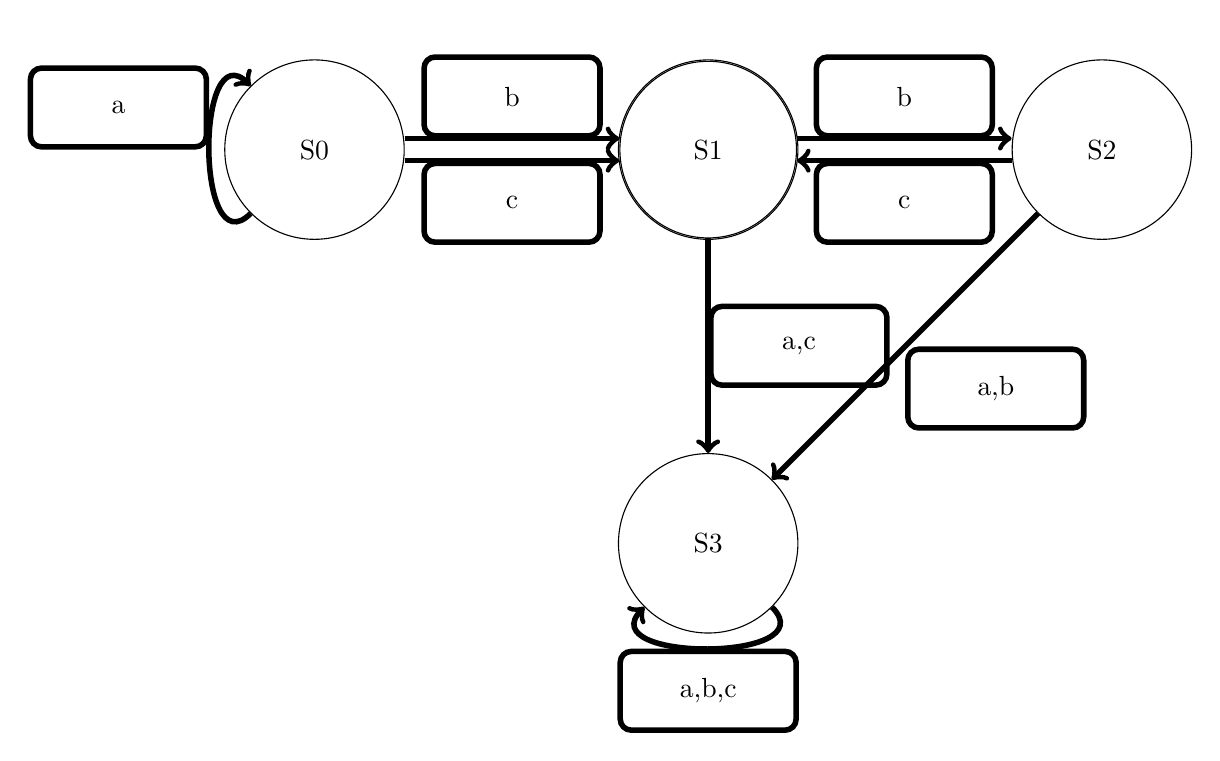
\begin{tikzpicture}
  	\def \n {5};
  	\node[circle, minimum width=1cm, draw=black](S0) at (0,\n) {S0};
  	\node[circle, minimum width=1cm, draw=black](S1) at (\n,\n) {S1};
  	\node[circle, minimum width=1cm, draw=black](S2) at (2*\n,\n) {S2};
  	\node[circle, minimum width=1cm, draw=black](S3) at (\n,0) {S3};
  	\node[circle, minimum width=1.2cm, draw=black](S4) at (\n,\n) {};
  	
  	
  	\draw[->, line width=2pt] ([yshift= 4pt]S0.east) -- node[above] {b} ([yshift= 4pt]S4.west);
  	\draw[->, line width=2pt] ([yshift= -4pt]S0.east) -- node[below] {c} ([yshift= -4pt]S4.west);
  	\draw[->, line width=2pt] (S0.south west) .. controls ([xshift= -20pt, yshift=-20pt]S0.south west) and ([xshift= -20pt, yshift= 20pt]S0.north west) .. node[above left] {a} (S0.north west);
  	
  	\draw[->, line width=2pt] ([yshift=4pt]S4.east) -- node[above] {b} ([yshift=4pt]S2.west);
  	\draw[->, line width=2pt] (S4.south) -- node[right] {a,c} (S3.north);
  	
  	\draw[->, line width=2pt] ([yshift=-4pt]S2.west) -- node[below] {c} ([yshift=-4pt]S4.east);
  	\draw[->, line width=2pt] (S2.south west) -- node[below right] {a,b} (S3.north east);
  	
  	\draw[->, line width=2pt] (S3.south east) .. controls ([xshift= 20pt, yshift = -20pt]S3.south east) and ([yshift= -20pt, xshift = -20pt]S3.south west) .. node[below] {a,b,c} (S3.south west);
  	\end{tikzpicture}
  	\caption*{State Transition Diagram}
  \end{figure}
  
  \noindent
  \marginnote{4.4.2.4}A regular language is a language that can be represented by a regular expression, thus will also be accepted by a finite state machine
  
\subsection{Context-free Languages}
  
  \noindent
  \marginnote{4.4.3.1}Context-free languages are languages that are defined by context-free grammars, which in turn are simply a set of rules which defines what strings are possible in a given language. We often find that languages are too complex to be represented by a regular expression or a finite state machine, thus context-free grammars are useful in these situations (e.g. try formulating a regular expression for a palindrome).
  
  Backus-Naur form is a notation we can use to describe context free grammars, thus describing the syntax of a program. There a few characters that are important within Backus-Naur Form:
  \begin{itemize}
  	\item <>
	  	\subitem The name within the curly bracket defines a non-terminal expression, that is an expression that can be broken down further. For example in the expression <digits>::=0|1|2|3|4|5|6|7|8|9 , <digits> would be a non-terminal, and the digits from 0 to 9 would be terminal as they can't be broken down any further.
  	\item ::=
	  	\subitem This is used to say how non-terminal expressions are defined
  	\item |
	  	\subitem This is a way of breaking up several parts of an expression, an 'or' of the different parts.
  \end{itemize}
  
  To give a simple example which defines decimals would be as follows
  <decimal> ::= <integer> "." <integer>
  <integer> ::= <digit> | <digit> <integer>
  <digit> ::= 0|1|2|3|4|5|6|7|8|9
  
  This shows that a decimal is 2 integers separated by a decimal point, an integer is either just a digit, or a digit followed by an integer (showing how context free grammars can be recursive), and a digit is defined as any natural number from 0 to 9.
  
  This can also be described using a syntax diagram, arrows show possible choices, ellipses show terminal expressions, and rectangles show non-terminal expressions. For example, the syntax diagrams for the above BNFs would be:
  
  \includegraphics[scale=0.4]{Syntax-Diagram}
  
\subsection{Classification of Algorithms}
  
  \noindent
  \marginnote{4.4.4.1}In computer science we often derive several algorithms in order to solve the same problem. It is useful to have a way for us to compare these algorithms either time-wise (how ling the algorithm takes) or space-wise (how much memory does the algorithm use).\\ \\
  \noindent
  \marginnote{4.4.4.2}In order to understand Big O-notation, you need to understand some basic functions (as well as some random related facts), the first thing is domain and co-domain. The domain is the set from which all the values that you can input into a function are taken and the co-domain is the set from which all of the output values can be taken. If you do A-level maths, it is similar to the concept of the range, however the co-domain can be larger than the range (the range is a subset of the co-domain). For example, take the function $f(x)=x^2$ (or $f: x \mapsto x^2$ written slightly differently) it has the domain $\mathbb{R}$ as you can put in any real number, and it can have co-domain $\mathbb{R}$ as all of its outputs are real numbers, you can see how this can be different to range, as the range would be $\{x \mid x \in \mathbb{R} \wedge x \geq 0\} = \mathbb{R}_0^+$. Often to fully define a function, they will state the domain and co-domain of a function in the following way, $f: \mathbb{R} \mapsto \mathbb{R}$, so if we wanted to define a new function $g(x)$ that produces the same output as $f(x)$ but has a different co-domain, we may say $g: \mathbb{R} \mapsto \mathbb{R}_0^+ \\ g: x \mapsto x^2$ and this has co-domain $\mathbb{R}_0^+$
  
  For this section, you also need to know some general graph functions:
  \begin{itemize}
  	\item Linear, this would be a graph of the form y = ax + b, for example $y = 2x+3$
  	
  	\begin{tikzpicture}[scale=0.6, every node/.style={transform shape}]
  	[line cap=round,line join=round,>=triangle 45,x=1cm,y=1cm]
  	\draw [color=cqcqcq,, xstep=1cm,ystep=1cm] (-4.3,-5.9) grid (9.46,6.3);
  	\draw[->,color=black] (-4.3,0) -- (9.46,0);
  	\foreach \x in {-4,-3,-2,-1,1,2,3,4,5,6,7,8,9}
  	\draw[shift={(\x,0)},color=black] (0pt,2pt) -- (0pt,-2pt) node[below] {\footnotesize $\x$};\draw[->,color=black] (0,-5.9) -- (0,6.3);
  	\foreach \y in {-5,-4,-3,-2,-1,1,2,3,4,5,6}
  	\draw[shift={(0,\y)},color=black] (2pt,0pt) -- (-2pt,0pt) node[left] {\footnotesize $\y$};
  	\draw[color=black] (0pt,-10pt) node[right] {\footnotesize $0$};\clip(-4.3,-5.9) rectangle (9.46,6.3);
  	\draw (-4.45,-5.9) -- (1.65,6.3);\end{tikzpicture}  	
  	
  	\item Polynomial - An expression in terms of variable with integer powers greater than or equal to 1. If the largest power is 0 then it is constant ($a$), 1 then it is linear ($ax+b$), 2 then it is quadratic ($ax^2 + bx + c$), 3 then it is cubic ($ax^3 + bx^2 + cx +d$), 4 quartic, 5 quintic, etc. Below are examples of a quadratic and cubic expressions with forms $y=x^2$ and $y=x^3-x$ respectively.
  	
  	\begin{tikzpicture}
  	[line cap=round,line join=round,>=triangle 45,x=1cm,y=1cm]
  	\draw [color=cqcqcq,, xstep=1cm,ystep=1cm] (-4.78996590159948,-2.0122769043830115) grid (5.077682925072191,3.6322654307068283);
  	\draw[->,color=black] (-4.78996590159948,0) -- (5.077682925072191,0);
  	\foreach \x in {-4,-3,-2,-1,1,2,3,4,5}
	  	\draw[shift={(\x,0)},color=black] (0pt,2pt) -- (0pt,-2pt) node[below] {\footnotesize $\x$};
  	\draw[->,color=black] (0,-2.0122769043830115) -- (0,3.6322654307068283);
  	\foreach \y in {-2,-1,1,2,3}
	  	\draw[shift={(0,\y)},color=black] (2pt,0pt) -- (-2pt,0pt) node[left] {\footnotesize $\y$};
  	\draw[color=black] (0pt,-10pt) node[right] {\footnotesize $0$};
  	\clip(-4.78996590159948,-2.0122769043830115) rectangle (5.077682925072191,3.6322654307068283);
  	\draw[smooth,samples=100,domain=-4.78996590159948:5.077682925072191] plot(\x,{(\x)^(2)});
  	\draw[line width=1.2pt,color=ccqqqq,smooth,samples=100,domain=-4.78996590159948:5.077682925072191] plot(\x,{((\x)^(2)-1)*(\x)});
  	\end{tikzpicture}
  	
  	\item Exponential - This an expression of the form $a \times b ^ x$ where $a$ and $b$ are constants. Below is the function $3^x$:
  	
  	\begin{tikzpicture}[scale=0.6, every node/.style={transform shape}]
  	[line cap=round,line join=round,>=triangle 45,x=1cm,y=1cm]
  	\draw [color=cqcqcq,, xstep=1cm,ystep=1cm] (-9.497184600752878,-0.7865459958507308) grid (3.5635447439440724,8.978100233465273);
  	\draw[->,color=black] (-9.497184600752878,0) -- (3.5635447439440724,0);
  	\foreach \x in {-9,-8,-7,-6,-5,-4,-3,-2,-1,1,2,3}
	  	\draw[shift={(\x,0)},color=black] (0pt,2pt) -- (0pt,-2pt) node[below] {\footnotesize $\x$};
  	\draw[->,color=black] (0,-0.7865459958507308) -- (0,8.978100233465273);
  	\foreach \y in {,1,2,3,4,5,6,7,8}\draw[shift={(0,\y)},color=black] (2pt,0pt) -- (-2pt,0pt) node[left] {\footnotesize $\y$};
	  	\draw[color=black] (0pt,-10pt) node[right] {\footnotesize $0$};
  	\clip(-9.497184600752878,-0.7865459958507308) rectangle (3.5635447439440724,8.978100233465273);
  	\draw[smooth,samples=100,domain=-9.497184600752878:3.5635447439440724] plot(\x,{3^((\x))});
  	\end{tikzpicture}
  	
  	\item Logarithmic, this is an expression of the form $y=\log_a(x)$ where a is a constant. The definition of a log is the solution $y$ to $b^y=x$, which means if $b^y=x$ then $y=\log_b(x)$. In other words its the power you have to raise a number to, to achieve another number. For example, if $2^x=128$, then we can see that $x = 7$, therefore $x = \log_2(128)=7$. The graph below shows $y=\log_{10}(x)$
  	
  	\begin{tikzpicture}[scale=0.6, every node/.style={transform shape}]
  	[line cap=round,line join=round,>=triangle 45,x=1cm,y=1cm]
  	\draw [color=cqcqcq,, xstep=1cm,ystep=1cm] (-0.9433339033525788,-7.8386188238055805) grid (13.423468375814059,2.902492028442017);
  	\draw[->,color=black] (-0.9433339033525788,0) -- (13.423468375814059,0);
  	\foreach \x in {,1,2,3,4,5,6,7,8,9,10,11,12,13}
  	\draw[shift={(\x,0)},color=black] (0pt,2pt) -- (0pt,-2pt) node[below] {\footnotesize $\x$};
  	\draw[->,color=black] (0,-7.8386188238055805) -- (0,2.902492028442017);
  	\foreach \y in {-7,-6,-5,-4,-3,-2,-1,1,2}
  	\draw[shift={(0,\y)},color=black] (2pt,0pt) -- (-2pt,0pt) node[left] {\footnotesize $\y$};
  	\draw[color=black] (0pt,-10pt) node[right] {\footnotesize $0$};
  	\clip(-0.9433339033525788,-7.8386188238055805) rectangle (13.423468375814059,2.902492028442017);
  	\draw[smooth,samples=1000,domain=1e-4:13.423468375814059] plot(\x,{ln((\x))/ln(10)});
  	\end{tikzpicture}
  	
  \end{itemize}
  
  Another thing you need to know is n factorial ($n!$). n factorial is equal to the product of all positive integers less than or equal to $n$, so $n!=n \times (n-1) \times (n-2) \times \dots \times 3 \times 2 \times 1$. factorial is used for when you want to find the number of ways a set can be ranged, the number of permutations of a set. To show you how, if we want to find all of the permutations of the word ``dog'' we would find $6=3!$, to list them all: dog, dgo, odg, ogd, gdo, god. To get the logic behind it, think about it this way, there are 3 ways to pick the first letter, then 2 to pick the second, then only one option left for the last, we get $3 \times 2 \times 1 = 3! = 6$ permutations, for a set with 4 elements, you have 4 choices, then 3 choices, then 2 choices, then 1 choice, giving you $4 \times 3 \times 2 \times 1 =  4! = 24$ permutations, for a set with 5 elements $5 \times 4 \times 3 \times 2 \times 1 = 5! 120$ permutations. This pattern goes on, so a set of $n$ elements has $n!$ permutations.\\ \\
  \noindent
  \marginnote{4.4.4.3}Big O notation is a way to describe an algorithm time-wise or space-wise. Big O notation has 5 main classifications in terms of time complexity:
  \begin{itemize}
  	\item Constant Time ($O(1)$)
	  	\subitem This is an algorithm that will always run in the same amount of time, no matter the size of the input. An example is accessing an array, as you get the value by referring directly to its address, thus no matter the size of the array, it will always take the same amount of time to carry out this process.
  	\item Linear Time ($O(N)$)
	  	\subitem This is an algorithm that grows proportionally to the size of the input. E.g. if the size of the input doubles, the amount of time the algorithm may also doubles. If you were to graph the length of time the algorithm takes against the size of input, you would end up with a linear function, so the above example may not necessarily be true if the graph made was $y=2x$, then is the size of the input doubled, the time taken would quadruple. A for loop over every element once will create an algorithm of linear time.
  	\item Polynomial Time ($O(N^k)$ where $k$ is a positive integer constant greater than 2)
	  	\subitem This is an algorithm that's time complexity can be upper bounded by a polynomial expression in terms of the size of the input, for the example, if the algorithm's time complexity can be expressed as $4n^2 + 6n - 4$, then in big O notation it can be written as $O(N^2)$. This can occur when iterative techniques are used, or when nested loops are used to iterate over elements, e.g. bubble sort.
  	\item Exponential Time ($O(k^N)$ where $k$ is a positive constant)
	  	\subitem This is an algorithm that's time complexity can be upper bounded by an exponential expression. Problems that require Algorithms of this time complexity to solve are called intractable problems as they become quite unwieldy as the size of the input increases.  	
  	\item Logarithmic Time ($O(\log(N))$)
	  	\subitem This is an algorithm that's time complexity can be upper bounded by an logarithmic expression. These time complexities often show up when working on a binary tree, or when performing a binary search.
  \end{itemize}
  
  The order of time complexity from best to worst is as follows (if you want to convince yourself of this, plot graphs of each on top of each other)
  \begin{enumerate}
  	\item Constant Time
  	\item Logarithmic Time
  	\item Linear Time
  	\item Polynomial Time
  	\item Exponential time
  \end{enumerate}
  
  When trying to derive the time complexity of the algorithm, consider the following:
  \begin{itemize}
  	\item Algorithms that require no data, and are simple assignment or comparisons, are linear time
  	\item Algorithms that feature a loop over all of the inputs, are linear.
  	\item Algorithms that feature multiple nested loops, all iterating over the inputs are polynomial time. The number of nested loops, indicate the order of the polynomial. e.g. bubble sort has 2 nested loops therefore it is $O(N^2)$, if we were to add a nested loop that printed the list after every stage, it would become $O(N^3)$.
  	\item Algorithms that use recursion may have exponential time complexity (not always true, as shown with the merge sort)
  	\item Splitting data into multiple pats, then performing actions on these parts, then repeating this, is often of logarithmic time complexity
  \end{itemize}
  
  \noindent
  \marginnote{4.4.4.4}In reality, we have limits to what we can do with an algorithm, such as the hardware (limits to RAM, and ROM), as well as the complexity of the algorithm, which limit what we can compute.\\ \\
  \noindent 
  \marginnote{4.4.4.5}There are two ways to classify a problem:
  \begin{itemize}
  	\item Tractable
	  	\subitem Problems that have algorithmic solutions that are of polynomial time complexity or less
  	\item Intractable
	  	\subitem Problems that do not have algorithmic solutions that are of polynomial time complexity or less. To solve these problems, often a heuristic is used, this is when you use some sort of measure to guess a solution, then use an algorithm to improve your initial guess. An example is the travelling salesman problem, which is to find the shortest route to visit all of the nodes in a weighted connected graph.
  \end{itemize}
  
  \noindent
  \marginnote{4.4.4.6}There are problems that exist that cannot be solved algorithmically, meaning no matter how powerful your computer is, the problem has no algorithm solutions.
  
  \noindent
  \marginnote{4.4.4.7}The Halting Problem is an example of a problem that cannot be solved algorithmically, as it would create a paradox. The halting problem is about trying to find an algorithm that can determine for all other algorithms whether it will end by feeding in this other algorithm. We can show that such an algorithm doesn't exist via a proof by contradiction. Let's assume that such an algorithm does exist and returns \verb|True| if the algorithm terminates, \verb|false| otherwise, we are going to feed in the following algorithm (let's call it the Anti-Halting Algorithm)
  
  \begin{verbatim}
IF the output of the halting algorithm is True:
    WHILE True:
        pass
    ENDWHILE
ELSE
    HALT
ENDIF
  \end{verbatim}Now we can look at the two cases that arise:
  \begin{enumerate}
  	\item The halting algorithm evaluates \verb|True|, meaning the anti-halting algorithm will halt
	  	\subitem Then the anti-halting algorithm will go into an infinite while loop, never halting
	\item The halting algorithm evaluates \verb|False|, meaning the anti-halting algorithm will not halt
		\subitem Then the anti-halting algorithm will halt
  \end{enumerate}
  
  Either way you will get some kind of contradiction, thus showing a halting algorithm cannot exist. Now you don't need to know the proof, but it is just good to understand why the halting problem is the way it is. We can gather 2 things from this:
  \begin{enumerate}
  	\item There are some problems that cannot be solved algorithmically (unsolvable problems)
  	\item There are some problems that cannot be solved in a reasonable time frame (intractable problems)
  \end{enumerate}

\subsection{A model of computation}
  \noindent
  \marginnote{4.4.5.1}A Turing Machine is a model of computation that is used to identify whether a problem is computable. 
  Here are the basics of the turing maching:
  \begin{itemize}
  	\item It is made up of a tape and a read/write head
  	\item the tape is made up of multiple cells that act as memory
  	\item Each cell will contain a symbol, often 0, 1 and the blank symbol (this can be many different things, including $\square$, $\diamondsuit$, or B)
  	\item The read/ write head can read from or write to what is currently underneath it (writing to it basically overwrites its current value), and starts at the left most not blank cell.
  	\item The tape can move left (L, $\leftarrow$) or right(R, $\rightarrow$), one cell at a time, meaning all cells are accessible to the read/write head.
  	\item The machine can halt at any point if it reaches a halting state (a state with no outgoing transitions) or has processed all of the input
  \end{itemize}
  The order in which the read/ write head performs its operations are as follows:
  \begin{enumerate}
  	\item \textbf{Read} the square currently underneath the read/write head
  	\item \textbf{Write} to the square currently underneath the read/write head
  	\item \textbf{Move} the read/write head left or right
  \end{enumerate} 
  To define a Turing machine, you need a start state, a halting state, ability to move the read/ write head, and a transition function, this defines what's to be written and what state to move to, given the current state and what has been read. There are 3 main ways to do this:
  \begin{itemize}
  	\item An instruction table
	  	\subitem this is a tabular way to show all of the transitions within a Turing machine, for example:
	  	\begin{table}[H]
	  		\begin{tabular}{| c | c | c | c | c |}\hline
	  			State & Read      & Write     & Move & Next State \\\hline
	  			S0    & 0         & 0         & R    & S0 \\\hline
	  			S0    & 1         & 1         & R    & S0 \\\hline
	  			S0    & $\square$ & $\square$ & L    & S1 \\\hline
	  			S1    & 0         & 0         & L    & S1 \\\hline
	  			S1    & 1         & 1         & L    & S2 \\\hline
	  			S1    & $\square$ & $\square$ & L    & S3 \\\hline
	  			S2    & 0         & 1         & L    & S2 \\\hline
	  			S2    & 1         & 0         & L    & S2 \\\hline
	  			S2    & $\square$ & $\square$ & L    & S3 \\\hline
	  		\end{tabular}
	  	\end{table}
  	\item A finite state machine
	  	\subitem A Turing machine can be represented as a finite state machine in the following way:
	  	
	  	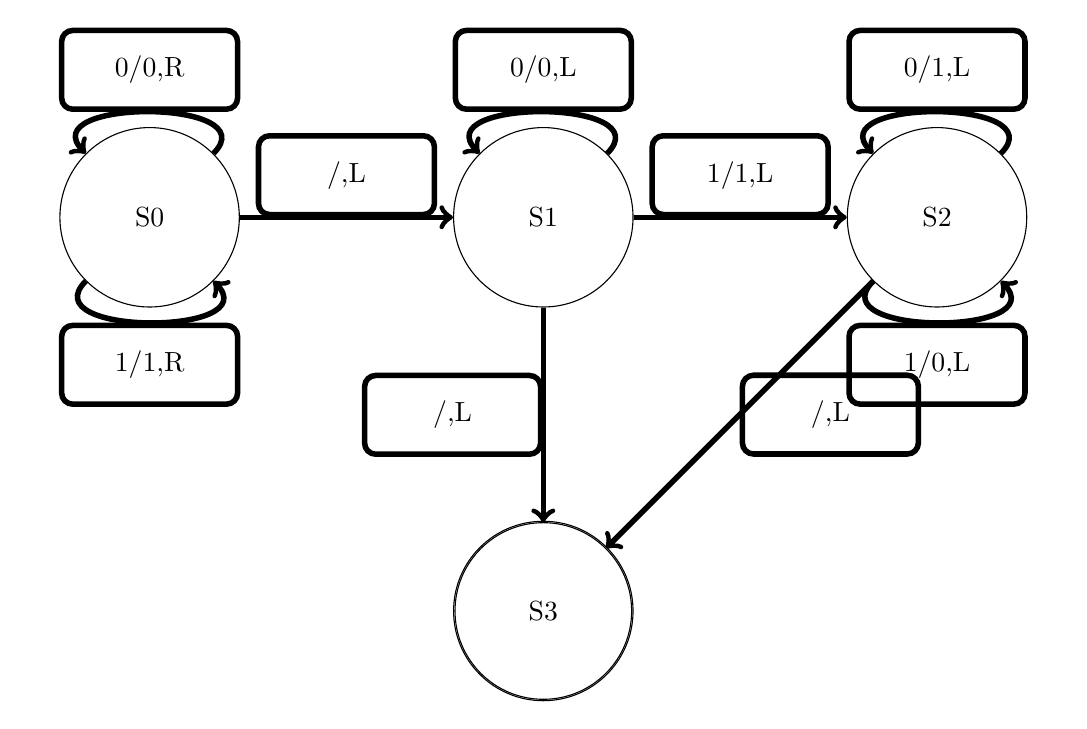
\begin{tikzpicture}
	  	\def \n {5};
	  	\node[circle, minimum width=1cm, draw=black](S1) at (0,\n) {S1};
	  	\node[circle, minimum width=1cm, draw=black](S0) at (-1*\n,\n) {S0};
	  	\node[circle, minimum width=1cm, draw=black](S2) at (\n,\n) {S2};
	  	\node[circle, minimum width=1cm, draw=black](S3) at (0,0) {S3};
	  	\node[circle, minimum width=1.2cm, draw=black](S4) at (0,0) {};
	  	
	  	\draw[->, line width=2pt] (S0.east) -- node[above] {$\square$/$\square$,L} (S1.west);
	  	\draw[->, line width=2pt] (S0.north east) .. controls ([xshift=20pt,yshift=20pt]S0.north east) and ([xshift=-20pt,yshift=20pt]S0.north west) .. node[above] {0/0,R} (S0.north west);
	  	\draw[->, line width=2pt] (S0.south west) .. controls ([xshift=-20pt,yshift=-20pt]S0.south west) and ([xshift=20pt,yshift=-20pt]S0.south east) .. node[below] {1/1,R} (S0.south east);
	  	
	  	\draw[->, line width=2pt] (S1.north east) .. controls ([xshift=20pt,yshift=20pt]S1.north east) and ([xshift=-20pt,yshift=20pt]S1.north west) .. node[above] {0/0,L} (S1.north west);
	  	\draw[->, line width=2pt] (S1.east) -- node[above] {1/1,L} (S2.west);
	  	\draw[->, line width=2pt] (S1.south) -- node[left] {$\square$/$\square$,L} (S4.north);
	  	
	  	\draw[->, line width=2pt] (S2.north east) .. controls ([xshift=20pt,yshift=20pt]S2.north east) and ([xshift=-20pt,yshift=20pt]S2.north west) .. node[above] {0/1,L} (S2.north west);
	  	\draw[->, line width=2pt] (S2.south west) .. controls ([xshift=-20pt,yshift=-20pt]S2.south west) and ([xshift=20pt,yshift=-20pt]S2.south east) .. node[below] {1/0,L} (S2.south east);
	  	\draw[->, line width=2pt] (S2.south west) -- node[right] {$\square$/$\square$,L} (S4.north east);
	  	\end{tikzpicture}
  	\item A list of transition rules
	  	\subitem A Turing machine can also be defined as a list of transition rules of the following form $\delta$(Current State, Input Symbol) = (Next State, Output Symbol, Movement). For example:
	  	\begin{itemize}
	  		\item $\delta$(S0,0) = (S0,0,R)
	  		\item $\delta$(S0,1) = (S0,1,R)
	  		\item $\delta$(S0,$\square$) = (S1,$\square$,L)
	  		\item $\delta$(S1,0) = (S1,0,L)
	  		\item $\delta$(S1,1) = (S2,1,L)
	  		\item $\delta$(S1,$\square$) = (S3,$\square$,L)
	  		\item $\delta$(S2,0) = (S2,1,L)
	  		\item $\delta$(S2,1) = (S2,0,L)
	  		\item $\delta$(S2,$\square$) = (S3,$\square$,L)
	  	\end{itemize}
  \end{itemize}
  
  All of the above examples define the same Turing machines, so let's see what the output is for the input of 10110.
  
  
  So it starts off as follows, in the state S0:
  
  \input{TM/TM1.txt}
  
  So then it reads 1, thus it writes 1, remains in S0, and moves right
  
  \input{TM/TM2.txt}
  
  Then it reads 0, thus it writes 0, remains in S0, and moves right
  
  \input{TM/TM3.txt}
  
  Then it reads 1, thus it writes 1, remains in S0, and moves right
  
  \input{TM/TM4.txt}
  
  Then it reads 1, thus it writes 1, remains in S0, and moves right
  
  \input{TM/TM5.txt}
  
  Then it reads 0, thus it writes 0, remains in S0, and moves right
  
  \input{TM/TM6.txt}
  
  Then it reads $\square$, thus it writes $\square$, Moves to the S1 state, and moves left
  
  \input{TM/TM7.txt}
  
  Then it reads 0, thus it writes 0, remains in S1, and moves left
  
  \input{TM/TM8.txt}
  
  Then it reads 1, thus it writes 1, Moves to the S2 state, and moves left
  
  \input{TM/TM9.txt}
  
  Then it reads 1, thus it writes 0, remains in S2, and moves left
  
  \input{TM/TM10.txt}
  
  Then it reads 0, thus it writes 1, remains in S2, and moves left
  
  \input{TM/TM11.txt}
  
  Then it reads 1, thus it writes 0, remains in S2, and moves left
  
  \input{TM/TM12.txt}
  
  Then it reads $\square$, thus it writes $\square$, Moves to the S3 state, and moves left. S3 is a halting state, therefore at this point the program stops, and the tape now reads 01010. The point of this Turing machine is to find the two's complement of the inputted string.
  
  A universal Turing machine is a machine that can simulate a Turing machine by reading a description of the machine along with the inputs of its tape. To put it another way, what it does is it takes in the description of another machine encoded into some sort of string, and from this is able to emulate the working of this machine onto an input, which would also be provided. Both the program and the data are stored on the tape, which is similar to the stored program concept, where the program and the data the program operates on are stored in the same location in memory. 
  
  Turing machines and Universal Turing machines are useful as they provide a model of computation which allows us to clearly define if a problem is computable, that is to say that if it can be solved using a universal Turing machine, then it is computable. Universal Turing machines are useful as you don't need to make a new machine for each problem, you just need the description of the machine, and the inputs you want it to work on.